\chapter{Resoconto attività di verifica } \label{ResocontoAttivitàDiVerifica}
In questa sezione si riportano gli esiti, descritti ed analizzati, di tutte le attività$_{\scaleto{G}{3pt}}$ di verifica svolte.
\section{Revisione dei Requisiti}  \label{ResocontoAttivitàDiVerificaRevisioneDeiRequisiti}
Tutta la documentazione sviluppata nella prima fase da consegnare per la Revisione dei Requisiti ha subito una meticolosa ed attenta revisione da parte dei Verificatori. Questi ultimi hanno seguito, in questa attività$_{\scaleto{G}{3pt}}$, per ogni documento, i metodi di \textit{Walkthrough$_G$} ed \textit{Inspection$_G$} relative all’analisi statica, stabilite nelle \textit{Norme di Progetto 2.0.0}. %% ?????? da rivedere quando scriviamo 3.4 sulle norme.
\subsection{Strategia adoperata per l’analisi statica dei documenti} \label{ResocontoAttivitàDiVerificaRevisioneDeiRequisitiStrategiaPerAnalisiStatica}
Il \textit{Verificatore} si è occupato di valutare la correttezza del documento, concentrandosi nell’individuare gli errori presenti in questo. Una volta individuati gli errori la strategia adottata è la seguente:
\begin{itemize}
	\item Correzione degli errori sia ortografici che sintattici, non fedeli alle norme tipografiche fissate nelle \textit{Norme di Progetto 2.0.0}.
\end{itemize}

\subsection{Esiti verifica} \label{ResocontoAttivitàDiVerificaRevisioneDeiRequisitiEsitiVerifica}
Per ciascun documento stilato si è calcolato l’indice di Gulpease$_{\scaleto{G}{3pt}}$. I risultati sono mostrati qui di seguito.
Per evitare risultati errati nel calcolo di tale indice, non si sono tenuti in considerazione:
\begin{itemize}
	\item il frontespizio di ogni documento;
	\item le eventuali tabelle presenti nel documenti;
	\item i diari delle modifiche di ogni documento.
\end{itemize}

\quad
\def\tabularxcolumn#1{m{#1}}
{\rowcolors{2}{RawSienna!90!RawSienna!20}{RawSienna!70!RawSienna!40}
	\begin{center}
		\renewcommand{\arraystretch}{1.4}
		\begin{tabularx}{11.50cm}{|c|c|c|}
			\hline
			\rowcolor{airforceblue}
			\textbf{Documento} & \textbf{Indice di Gulpease} & \textbf{Esito}\\
			\hline
			\textit{Analisi dei Requisiti 1.0.0} & 96  & \textit{Superato}\\
			\hline
			\textit{Norme di Progetto 1.0.0} & 75 & \textit{Superato}\\
			\hline
			\textit{Studio di Fattibilità 1.0.0} & 70 & \textit{Superato}\\
			\hline
			\textit{Piano di Progetto 1.0.0} & 77 & \textit{Superato}\\
			\hline
			\textit{Piano di Qualifica 1.0.0} & 80 & \textit{Superato}\\
			\hline
		\end{tabularx}
		\captionof{table}{\textbf{Elenco Indici di Gulpease$_{\scaleto{G}{3pt}}$ dei documenti versione v1.0.0}}
	\end{center}


\begin{figure}[!h]
	\begin{center}
		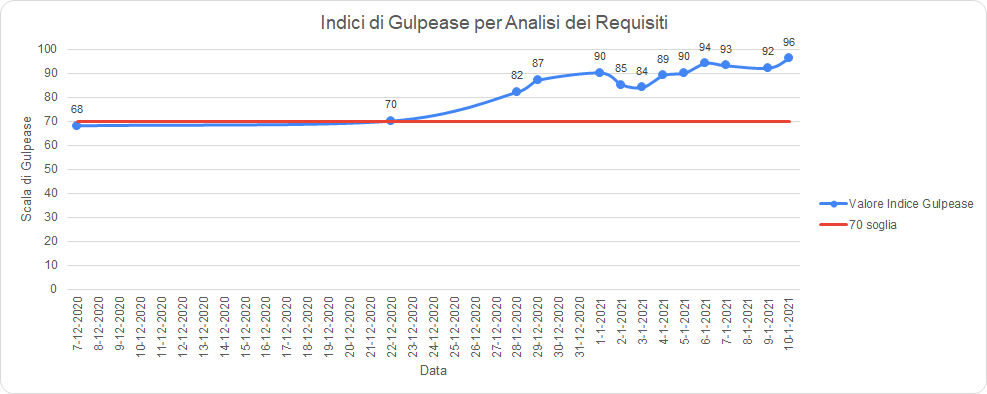
\includegraphics[width=1\linewidth]{../immagini/IndexGulpeaseAdR.png}
		\caption{\textbf{Andamento Indice di Gulpease$_{\scaleto{G}{3pt}}$ Analisi dei Requisiti fino a RR}}
	\end{center}
\end{figure}

\begin{figure}[!h]
	\begin{center}
		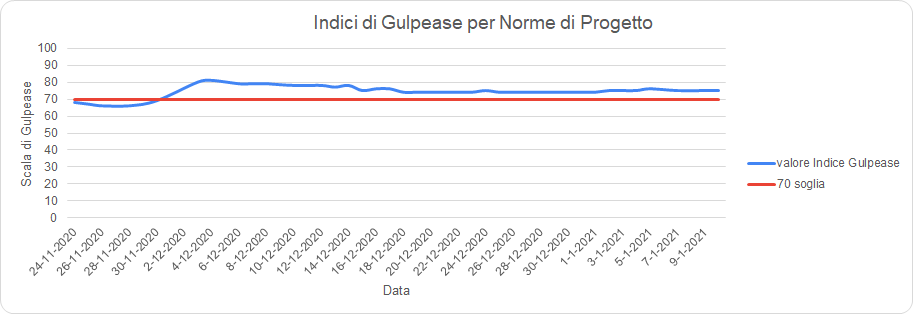
\includegraphics[width=1\linewidth]{../immagini/IndexGulpeaseNdP.png}
		\caption{\textbf{Andamento Indice di Gulpease$_{\scaleto{G}{3pt}}$ Norme di Progetto fino a RR}}
	\end{center}
\end{figure}

\begin{figure}[!h]
	\begin{center}
		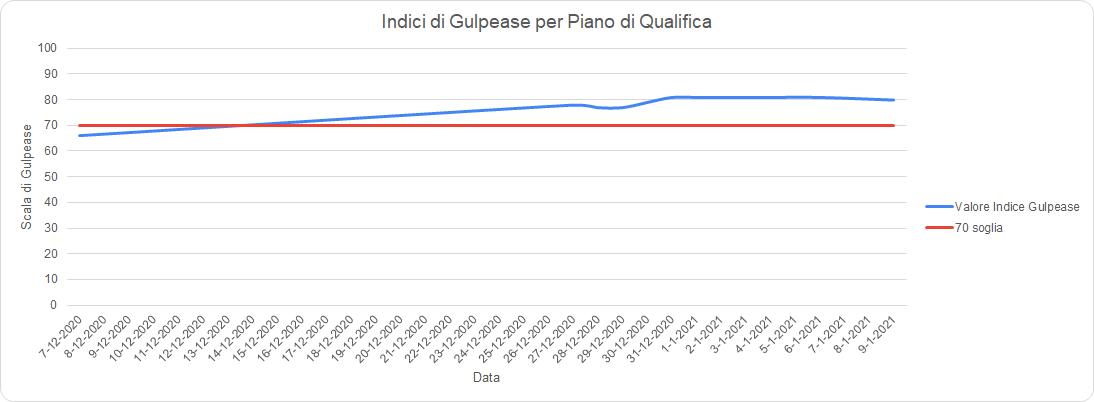
\includegraphics[width=1\linewidth]{../immagini/IndexGulpeasePdQ.png}
		\caption{\textbf{Andamento Indice di Gulpease$_{\scaleto{G}{3pt}}$ Piano di Qualifica fino a RR}}
	\end{center}
\end{figure}

\begin{figure}[!h]
	\begin{center}
		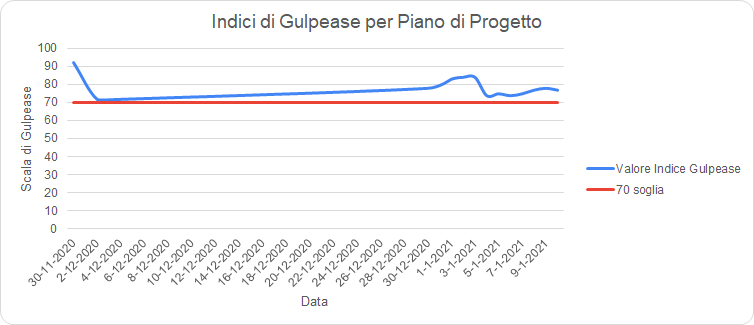
\includegraphics[width=1\linewidth]{../immagini/IndexGulpeasePdP.png}
		\caption{\textbf{Andamento Indice di Gulpease$_{\scaleto{G}{3pt}}$ Piano di Progetto fino a RR}}
	\end{center}
\end{figure}

\begin{figure}[H]
	\begin{center}
		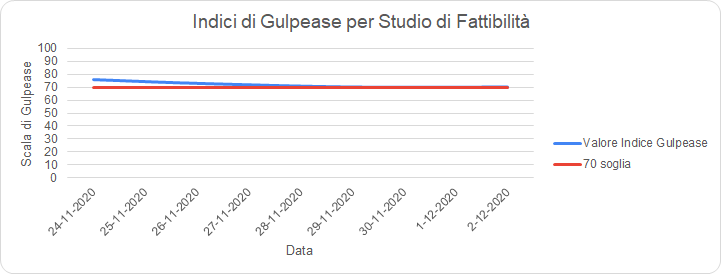
\includegraphics[width=1\linewidth]{../immagini/IndexGulpeaseSdF.png}
		\caption{\textbf{Andamento Indice di Gulpease$_{\scaleto{G}{3pt}}$ Studio di Fattibilità fino a RR}}
	\end{center}
\end{figure}

Per quanto riguarda gli Indici di Gulpease$_{\scaleto{G}{3pt}}$ dei verbali si è deciso di rappresentare i risultati in forma tabellare.
Questo in quanto il verbale viene scritto tutta in una volta, quindi utilizzare un grafico temporale risulta non idoneo.
\quad
\def\tabularxcolumn#1{m{#1}}
{\rowcolors{2}{RawSienna!90!RawSienna!20}{RawSienna!70!RawSienna!40}
	\begin{center}
		\renewcommand{\arraystretch}{1.4}
		\begin{tabularx}{11.65cm}{|c|c|c|}
			\hline
			\rowcolor{airforceblue}
			\textbf{Documento} & \textbf{Indice di Gulpease} & \textbf{Esito}\\
			\hline
			\textit{verbale\_interno\_28-10-2020} & 100  & \textit{Superato}\\
			\hline
			\textit{verbale\_interno\_19-11-2020} & 100 & \textit{Superato}\\
			\hline
			\textit{verbale\_interno\_24-11-2020} & 99 & \textit{Superato}\\
			\hline
			\textit{verbale\_interno\_04-12-2020} & 98 & \textit{Superato}\\
			\hline
			\textit{verbale\_esterno\_17-12-2020} & 99 & \textit{Superato}\\
			\hline
			\textit{verbale\_interno\_29-12-2020} & 100 & \textit{Superato}\\
			\hline
			\textit{verbale\_interno\_03-01-2021} & 100 & \textit{Superato}\\
			\hline
			\textit{verbale\_interno\_06-01-2021} & 100 & \textit{Superato}\\
			\hline
		\end{tabularx}
		\captionof{table}{\textbf{Elenco Indici di Gulpease$_{\scaleto{G}{3pt}}$ dei verbali versione v1.0.0}}
	\end{center}

\section{Revisione di Progettazione} \label{ResocontoAttivitàDiVerificaRevisioneDiProgettazione}
Tutta la documentazione da consegnare per la Revisione dei Progettazione ha subito una meticolosa ed attenta revisione da parte dei Vericatori. Questi ultimi
hanno seguito, per ogni documento, i metodi di \textit{Walkthrough$_G$} ed \textit{Inspection$_G$} relative all'analisi statica, stabilite nelle \textit{Norme di Progetto 2.0.0}.

\subsection{Verifiche di processo} \label{RevisioneDiProgettazioneVerificheDiProcesso}
\begin{center}
 \begin{figure}[H]
	 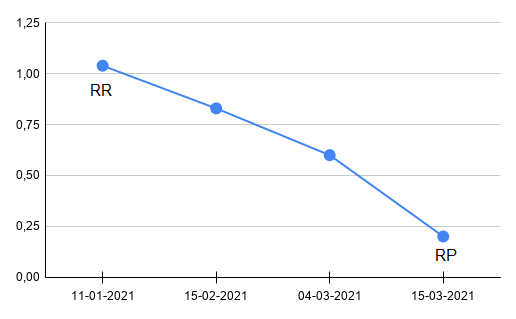
\includegraphics[width=1\linewidth]{../immagini/Metriche/MQPS05.png}
	 \caption{\textbf{MQPS05}}
 \end{figure}
\end{center}
Il grafico indica la variazione di giorni di lavoro, dove l'asse dello zero individua il rispetto dei tempi di lavoro. Da questo si evidenzia come in entrambe le fasi ci sia una maggiorazione di giorni di lavoro rispetto a quelli preventivati. Anche se presente una maggiorazione si può notare come il gruppo sia riuscito ad ottimizzare il lavoro dalla \textit{Revisione dei Requisiti} per diminuire il più possibile questo difetto.
 \subsection{Verifiche di prodotto} \label{ResocontoAttivitàDiVerificaRevisioneDiProgettazioneVerificheDiProdotto}
\subsubsection{Strategia adoperata per l’analisi statica dei documenti} \label{ResocontoAttivitàDiVerificaRevisioneDiProgettazioneVerificheDiProdottoStrategiaPerAnalisiStatica}
La strategia adoperata per l’analisi statica dei documenti per la \textit{Revisione di Progettazione} è la medesima di quella descritta in \S~\ref{ResocontoAttivitàDiVerificaRevisioneDeiRequisitiStrategiaPerAnalisiStatica}.
\paragraph{Esiti Verifica} \label{ResocontoAttivitàDiVerificaRevisioneDiProgettazioneVerificheDiProdottoStrategiaPerAnalisiStaticaEsitiVerifica}
Per ciascun documento stilato si è calcolato l’indice di Gulpease$_{\scaleto{G}{3pt}}$. I risultati sono mostrati qui di seguito.
Per evitare risultati errati nel calcolo di tale indice, non si sono tenuti in considerazione:
\begin{itemize}
	\item il frontespizio di ogni documento;
	\item le eventuali tabelle presenti nel documenti;
	\item i diari delle modifiche di ogni documento.
\end{itemize}
\quad
\def\tabularxcolumn#1{m{#1}}
{\rowcolors{2}{RawSienna!90!RawSienna!20}{RawSienna!70!RawSienna!40}
	\begin{center}
		\renewcommand{\arraystretch}{1.4}
		\begin{tabularx}{11.50cm}{|c|c|c|}
			\hline
			\rowcolor{airforceblue}
			\textbf{Documento} & \textbf{Indice di Gulpease} & \textbf{Esito}\\
			\hline
			\textit{Analisi dei Requisiti 3.0.0} & 92  & \textit{Superato}\\
			\hline
			\textit{Norme di Progetto 2.0.0} & 86 & \textit{Superato}\\
			\hline
			\textit{Piano di Progetto 2.0.0} & 79 & \textit{Superato}\\
			\hline
			\textit{Piano di Qualifica 2.0.0} & 84 & \textit{Superato}\\
			\hline
		\end{tabularx}
		\captionof{table}{\textbf{Elenco Indici di Gulpease$_{\scaleto{G}{3pt}}$ dei documenti per la RP}}
	\end{center}

\begin{figure}[!h]
	\begin{center}
		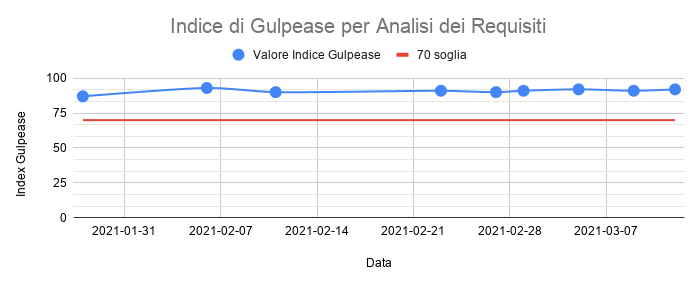
\includegraphics[width=1\linewidth]{../immagini/gulpeaseRP/IndicediGulpease perAnalisiDeiRequisiti.png}
		\caption{\textbf{Andamento Indice di Gulpease$_{\scaleto{G}{3pt}}$ Analisi dei Requisiti fino a RP}}
	\end{center}
\end{figure}

\begin{figure}[H]
	\begin{center}
		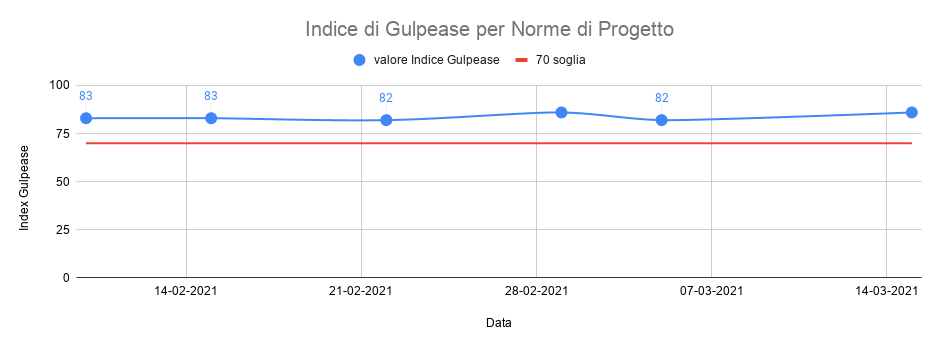
\includegraphics[width=1\linewidth]{../immagini/gulpeaseRP/IndicediGulpeaseperNormediProgetto.png}
		\caption{\textbf{Andamento Indice di Gulpease$_{\scaleto{G}{3pt}}$ Norme di Progetto fino a RP}}
	\end{center}
\end{figure}

\begin{figure}[H]
	\begin{center}
		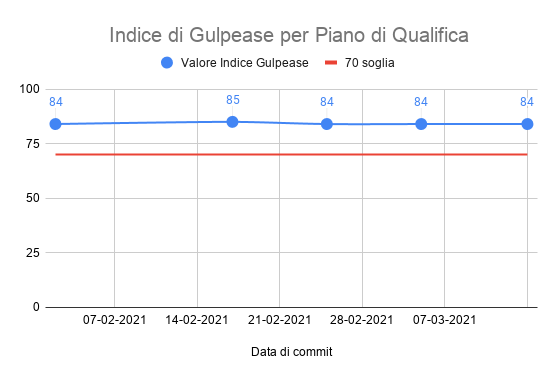
\includegraphics[width=0.9\linewidth]{../immagini/gulpeaseRP/indPdQ2.png}
		\caption{\textbf{Andamento Indice di Gulpease$_{\scaleto{G}{3pt}}$ Piano di Qualifica fino a RP}}
	\end{center}
\end{figure}

\begin{figure}[H]
	\begin{center}
		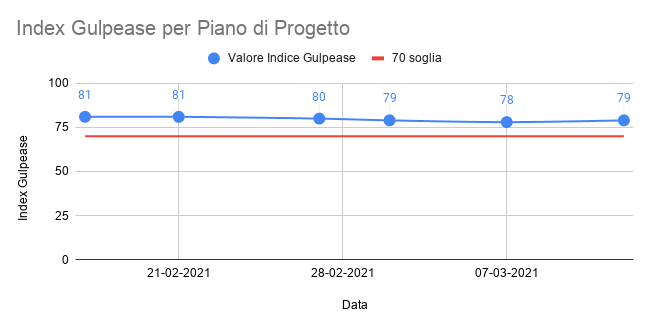
\includegraphics[width=0.9\linewidth]{../immagini/gulpeaseRP/indPdP2.png}
		\caption{\textbf{Andamento Indice di Gulpease$_{\scaleto{G}{3pt}}$ Piano di Progetto fino a RP}}
	\end{center}
\end{figure}

%ALTRI GRAFICI

Per quanto riguarda gli Indici di Gulpease$_{\scaleto{G}{3pt}}$ dei verbali si è deciso di rappresentare i risultati in forma tabellare.
Questo in quanto il verbale viene scritto tutta in una volta, quindi utilizzare un grafico temporale risulta non idoneo.
\quad
\def\tabularxcolumn#1{m{#1}}
{\rowcolors{2}{RawSienna!90!RawSienna!20}{RawSienna!70!RawSienna!40}
	\begin{center}
		\renewcommand{\arraystretch}{1.4}
		\begin{tabularx}{9.5cm}{|c|c|c|}
			\hline
			\rowcolor{airforceblue}
			\textbf{Documento} & \textbf{Indice di Gulpease} & \textbf{Esito}\\
			\hline
			\textit{v\_e\_28-01-2021} & 99 & \textit{Superato}\\
			\hline
			\textit{v\_i\_29-01-2021} & 98  & \textit{Superato}\\
			\hline
			\textit{v\_e\_02-02-2021} & 100 & \textit{Superato}\\
			\hline
			\textit{v\_e\_08-02-2021} & 100 & \textit{Superato}\\
			\hline
			\textit{v\_i\_10-02-2021} & 100 & \textit{Superato}\\
			\hline
			\textit{v\_i\_17-02-2021} & 99 & \textit{Superato}\\
			\hline
			\textit{v\_e\_25-02-2021} & 98 & \textit{Superato}\\
			\hline
			\textit{v\_i\_26-02-2021} & 100 & \textit{Superato}\\
			\hline

			\textit{v\_i\_08-03-2021} & 100 & \textit{Superato}\\
			\hline
		\end{tabularx}
		\captionof{table}{\textbf{Elenco Indici di Gulpease$_{\scaleto{G}{3pt}}$ dei verbali versione v1.0.0}}
	\end{center}

\section{Revisione di qualifica}\label{ResocontoAttivitàDiVerificaRevisioneDiQualifica}

\subsection{Esiti verifica}\label{ResocontoAttivitàDiVerificaRevisioneDiQualificaEsitiVerifica}